\documentclass{exam}
\usepackage{tasks}

\usepackage{amsmath,amssymb,amsfonts}
\usepackage{graphicx}
\usepackage{amsthm}
\usepackage[french]{babel}
\usepackage{enumitem}
\usepackage{currfile}

\usepackage{tikz}
\usetikzlibrary{calc}
\usepackage{qrcode}
\usepackage{mathrsfs}
\usepackage{enumitem}
\usepackage[french]{babel}
\usepackage[most]{tcolorbox}
\setlength{\parindent}{0cm}

\usepackage{multicol}
\newenvironment{clist}{
  \begin{center}
  \begin{inparaenum}}{
    \end{inparaenum}
\end{center}}

\pagestyle{empty}

\usepackage{geometry}
\geometry{left=1.5cm, right=1.5cm, top=1.5cm, bottom=1.5cm}

\makeatletter
\def\gap#1{%
  \setbox\@tempboxa\hbox{{\color{white}#1}}%
  \@tempdima\wd\@tempboxa
  \rlap{\unhbox\@tempboxa}%
  \hb@xt@\@tempdima{\dotfill}%
}
\makeatother

\theoremstyle{definition}
\newtheorem{exercice}{Exercice}


\begin{document}
\large

\vfill

\noindent{
  \Large
  \makebox[0pt][l]{\textbf{Première}}%
  \makebox[\textwidth][c]{\textbf{Bac blanc}}%
  \makebox[0pt][r]{\textbf{4h}}
}


\begin{center}
 \begin{tcolorbox}[hbox]
   \Large
   La \textbf{calculatrice} scientifique est \textbf{autorisée}. Veuillez \textbf{détailler vos calculs}.
 \end{tcolorbox}
\end{center}


%\noindent{\makebox[\textwidth]{Nom et prénom:\enspace\hrulefill}}

%\vspace{5mm}
%\noindent{\makebox[\textwidth]{Nom et prénom:\enspace\hrulefill}}

%\begin{center}
%\fbox{\fbox{\parbox{5.5in}{\centering
%Répondez dans les espaces fournis. Si vous n'avez plus de place, continuez sur le verso.}}}
%\end{center}

\section*{Partie A -- Suites.}

\begin{exercice}[30 min]
  \begin{enumerate}
    \item Pour chacune des suites suivantes, indiquer si elle est arithmétique ou géométrique, et préciser sa raison. Justifier si elle ne l'est pas.
      \begin{enumerate}
        \item $u_0 = 2, u_{n+1} = \dfrac{4 u_n}{3}$.
          %\item $u_n = 1.5 \times \left(\dfrac{2}{3}\right)^n$.
        \item $u_1 = 2, u_{n+1} = u_n + \dfrac{5}{3}$.
        \item $u_n = n^2 - 8n$.
      \end{enumerate}
    \item Pour chaque suite, déterminer ses variations (croissante, décroissante) sur $\mathbb{N}$.
    \item Pour chaque suite, exprimer sa forme explicite.
    \item Calculer les sommes suivantes:
      \begin{enumerate}
        \item $1+\dfrac{1}{2}+\dfrac{1}{4}+\dots+\dfrac{1}{4096}$.
        \item $5+9+13+\dots+493$.
      \end{enumerate}
  \end{enumerate}

\end{exercice}

\vfill

\begin{exercice}[40 min]
  Le 1\textsuperscript{er} janvier 2025, une grande entreprise compte \(1500\) employés.
  Une étude montre que lors de chaque année à venir, \(10\%\) de l'effectif de l'entreprise au 1\textsuperscript{er} janvier partira à la retraite au cours de l'année. Pour ajuster ses effectifs à ses besoins, l'entreprise embauche \(100\) jeunes dans l'année.

  Pour tout entier naturel \(n\), on appelle \(u_n\) le nombre d'employés de l'entreprise le 1\textsuperscript{er} janvier de l'année \((2025 + n)\).

  \begin{enumerate}
    \item Déterminer les trois premiers termes de la suite.
      Cette suite est-elle géométrique ? Arithmétique ? Justifier votre réponse.

    \item Donner la relation de récurrence entre \(u_{n+1}\) et \(u_n\).

    \item Pour tout entier naturel \(n\), on pose \(v_n = u_n - 1000\).
      Montrer que la suite \((v_n)\) est géométrique.

    \item En déduire l'expression de \((v_n)\) puis de \((u_n)\) en fonction de \(n\).

    \item Démontrer que pour tout entier naturel \(n\), on a :
      \[
        u_{n+1} - u_n \;=\; -50 \times 0{,}9^n.
      \]
      En déduire alors le sens de variation de la suite \(\bigl(u_n\bigr)\).

    \item Au 1\textsuperscript{er} janvier 2025, l'entreprise compte un sureffectif de \(300\) employés.
      À partir de quelle année, le contexte restant le même, l'entreprise ne sera-t-elle plus en sureffectif ?
  \end{enumerate}
\end{exercice}

\vfill

\newpage

\section*{Partie B -- Polynômes.}

\begin{exercice}[30 min]
  \begin{enumerate}
    \item[]
    \item On considère les fonctions polynôme suivantes :
      \begin{tasks}(2)[style=itemize]
        \task[ ] $f(x) = 2x^2 -5x + 3$.
        \task[ ] $g(x) = x^2 -x + 4$.
      \end{tasks}
      Pour chaque fonction :
      \begin{enumerate}
        \item Déterminer ses éventuelles racines, en déduire son éventuelle forme factorisée.
        \item Dresser son tableau de signes.
        \item Dresser son tableau de variations.
      \end{enumerate}
      %\item Dresser le tableau de signes de $2x^3 + 8x^2 + 8x$.
    \item Déterminez deux entiers naturels séparés de $101$ (par exemple $10$ et $111$) dont le produit est $24\,182$.
  \end{enumerate}
\end{exercice}

% Exercice 25
\begin{exercice}[30 min]
  ~\\
  \begin{minipage}{0.7\linewidth}
    On considère un carré $ABCD$ de côté $AB = 1$. $EFGH$ est un carré tel que :
    \begin{itemize}
      \item Les points $E$, $F$, $G$, $H$ appartiennent respectivement aux côtés $[AB]$, $[BC]$, $[CD]$ et $[AD]$.
      \item $AE = BF = CG = DH = x$ avec $0 \leq x \leq 1$.
    \end{itemize}
    Déterminer la valeur de $x$ pour laquelle l'aire du carré $EFGH$ est minimale.
  \end{minipage}
  \begin{minipage}{0.3\linewidth}
    \begin{center}
      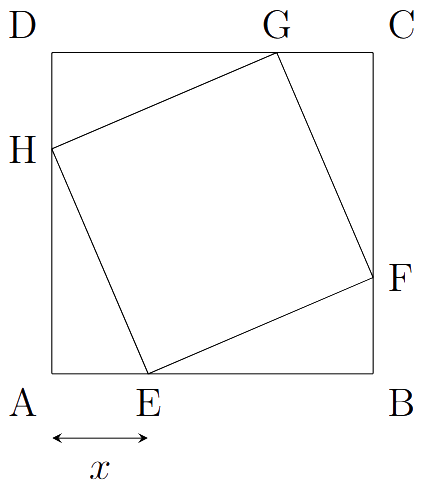
\includegraphics[width=0.7\linewidth]{swappy-20241230_104523.png}
    \end{center}
  \end{minipage}

\end{exercice}

\section*{Partie C -- Dérivation.}

\begin{exercice}{(10 min)}
  Pour chaque fonction $f$, déterminer $f'(x)$ en simplifiant au maximum.
  \begin{enumerate}
      % \item $f(x) = 2x^2 - x$
      % \item $f(x) = \dfrac{x^3}{3} + \dfrac{3}{x}$
      % \item $f(x) = \dfrac{3\sqrt{x}+1}{5}$
      % \item $f(x) = \dfrac{x}{\sqrt{x} - 1}$
      % \item $f(x) = \sqrt{2x - 4}$
      %\item $f(x) = -5x^2 + 5$
      %\item $f(x) = \dfrac{2x^3-1}{5}$
    \item $g(x) = \dfrac{4}{x} + \dfrac{2x^4}{4}$ définie et dérivable sur $\mathbb{R}^\star$.
    \item $f(x) = \dfrac{\sqrt{x}}{x + 1}$ définie sur $\mathbb{R}_+$ et dérivable sur $\mathbb{R}_+^\star$.
  \end{enumerate}
\end{exercice}

\begin{exercice}(40 min)
  ~\\
  \begin{minipage}{0.7\linewidth}
    On considère la parabole \(\mathcal{P}\) d'équation \(y = x^2\) et le point
    \[
      A \left(\dfrac{1}{2};\; \dfrac{5}{4}\right).
    \]
    On cherche à déterminer l'abscisse \(x\) du point \(M\) de la parabole le plus proche de \(A\).
  \end{minipage}
  \begin{minipage}{0.3\linewidth}
    \begin{center}
      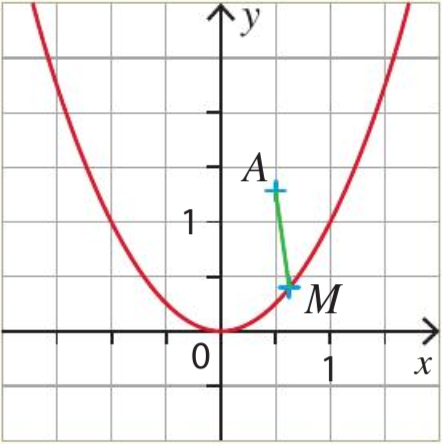
\includegraphics[width=0.7\linewidth]{swappy-20250206_115909.png}
    \end{center}
  \end{minipage}

  \begin{enumerate}
    \item Quelles sont les coordonnées du point \(M\), mobile sur la parabole \(\mathcal{P}\), en fonction de \(x\) ?

    \item Déterminer \(\mathrm{AM}^2\) en fonction de \(x\).

    \item On considère la fonction \(f\) définie sur \(\mathbb{R}\) par
      \[
        f(x) \;=\; x^4 \;-\; \dfrac{3}{2}\,x^2 \;-\; x \;+\; \dfrac{29}{16}.
      \]
      \begin{enumerate}
        \item Déterminer \(f'(x)\).
        \item Montrer que \(\displaystyle f'(x) = (\,x - 1\,)\,\left(4x^2 + 4x + 1\right)\).
        \item En déduire le signe de \(f'(x)\) puis établir le tableau de variation de \(f\).
      \end{enumerate}

    \item Répondre au problème posé : déterminer l'abscisse du point \(M\) de la parabole le plus proche de \(A\).
  \end{enumerate}
\end{exercice}

\end{document}